\documentclass{article}
\usepackage{graphicx} % Required for inserting images
    \setkeys{Gin}{width=\linewidth,totalheight=\textheight,keepaspectratio}
\usepackage{amsmath}

\title{Lecture 6 exercises}
\author{Group 4: Esther Müller, Eszter Szánthó, Hanna Hedman,\\ Rachel Angelyn Gunawan and Edward Karlsson}
\date{November 2023}

\begin{document}

\maketitle
\section*{Exercise 1}
\emph{Prove that $T''$ actually is a spanning tree.}
\vspace{0.4cm}
 
First let us check that $T''$ is connected: Let $u$ and $v$ be the two vertices $f$ is incident to. We note that by Lemma 2 we have that removing $f$ from $T'$ creates two separate trees $T_1$ and $T_2$ that are disconnected from each other. Since $e$ is part of a cycle with $f$ we have that there exists a walk between $u$ and $v$ containing $e$ that does not contain $f$. Without loss of generality we have by construction that $u \in V(T_1)$ and $v \in V(T_2)$. Then $e$ connects $T_1$ and $T_2$ giving us that $T''$ is connected.

Now we want to prove that $T''$ is acyclic. We have for any cycle in $T''$ that it has to go through $e$ since any cycle that does not go through $e$ would go through edges only in $T'$ meaning that we can find a cycle in $T'$. This contradicts $T'$ being a tree. However if $e$ is part of a cycle in $T''$ then there exists a trail between $u$ and $v$ that does not contain $e$. Since $u \in V(T_1)$ and $v \in V(T_2)$ any trail between them requires an edge between $T_1$ and $T_2$, which means that there exists and edge between them that is not $e$ in $T''$. This contradicts $T_1$ and $T_2$ being disconnected meaning that there can be no cycle in $T''$.

Lastly by construction $T''$ contains the same vertices as $T'$ meaning that it's a spanning subgraph.

Putting this together we have that $T''$ is connected, has no cycles and is a spanning subgraph of $G$ and therefore by definition a spanning tree.

\section*{Exercise 2}
\emph{Prove that this really is a tree. You can equivalently think of it as the union of all shortest paths between the root v and some other vertex. (This tree is called a shortest-path tree.)}
\vspace{0.4cm}

To show that this graph $T$ is a tree, we must prove that the graph contains no cycle and is connected.

By definition, there exist at least one shortest path between the root vertex $v$ and any other vertex, therefore we have a path between any vertex $u$ and vertex $w$ by combining the paths from $u$ to $v$ and $v$ to $w$. Thus the graph is connected.

Assume for contradiction that there is a cycle in the union of the shortest paths. For each vertex we pick the neighbour closest to the root as its parent. Suppose a cycle emerges when adding an edge to connect a certain vertex $w$ while picking the closest neighbour to the root. There has to be a vertex in this cycle that is furthest from the root which means that there is a vertex with two parents. (Otherwise, if every vertex would have one parent we would have a vertex that would be closer to the root than itself. This cannot hold.) Due to the definition of the algorithm we can only choose one vertex as the parent of another. 
Thus, having a vertex with more than one parent is a contradiction. Hence $T$ is acyclic and connected and therefore a tree.

\section*{Exercise 3}

\emph{Is it true that, under the assumption that all edges have different weights, no two spanning trees of a graph G have the same weight?}
\vspace{0.4cm}

\begin{figure}[h]
    \centering
    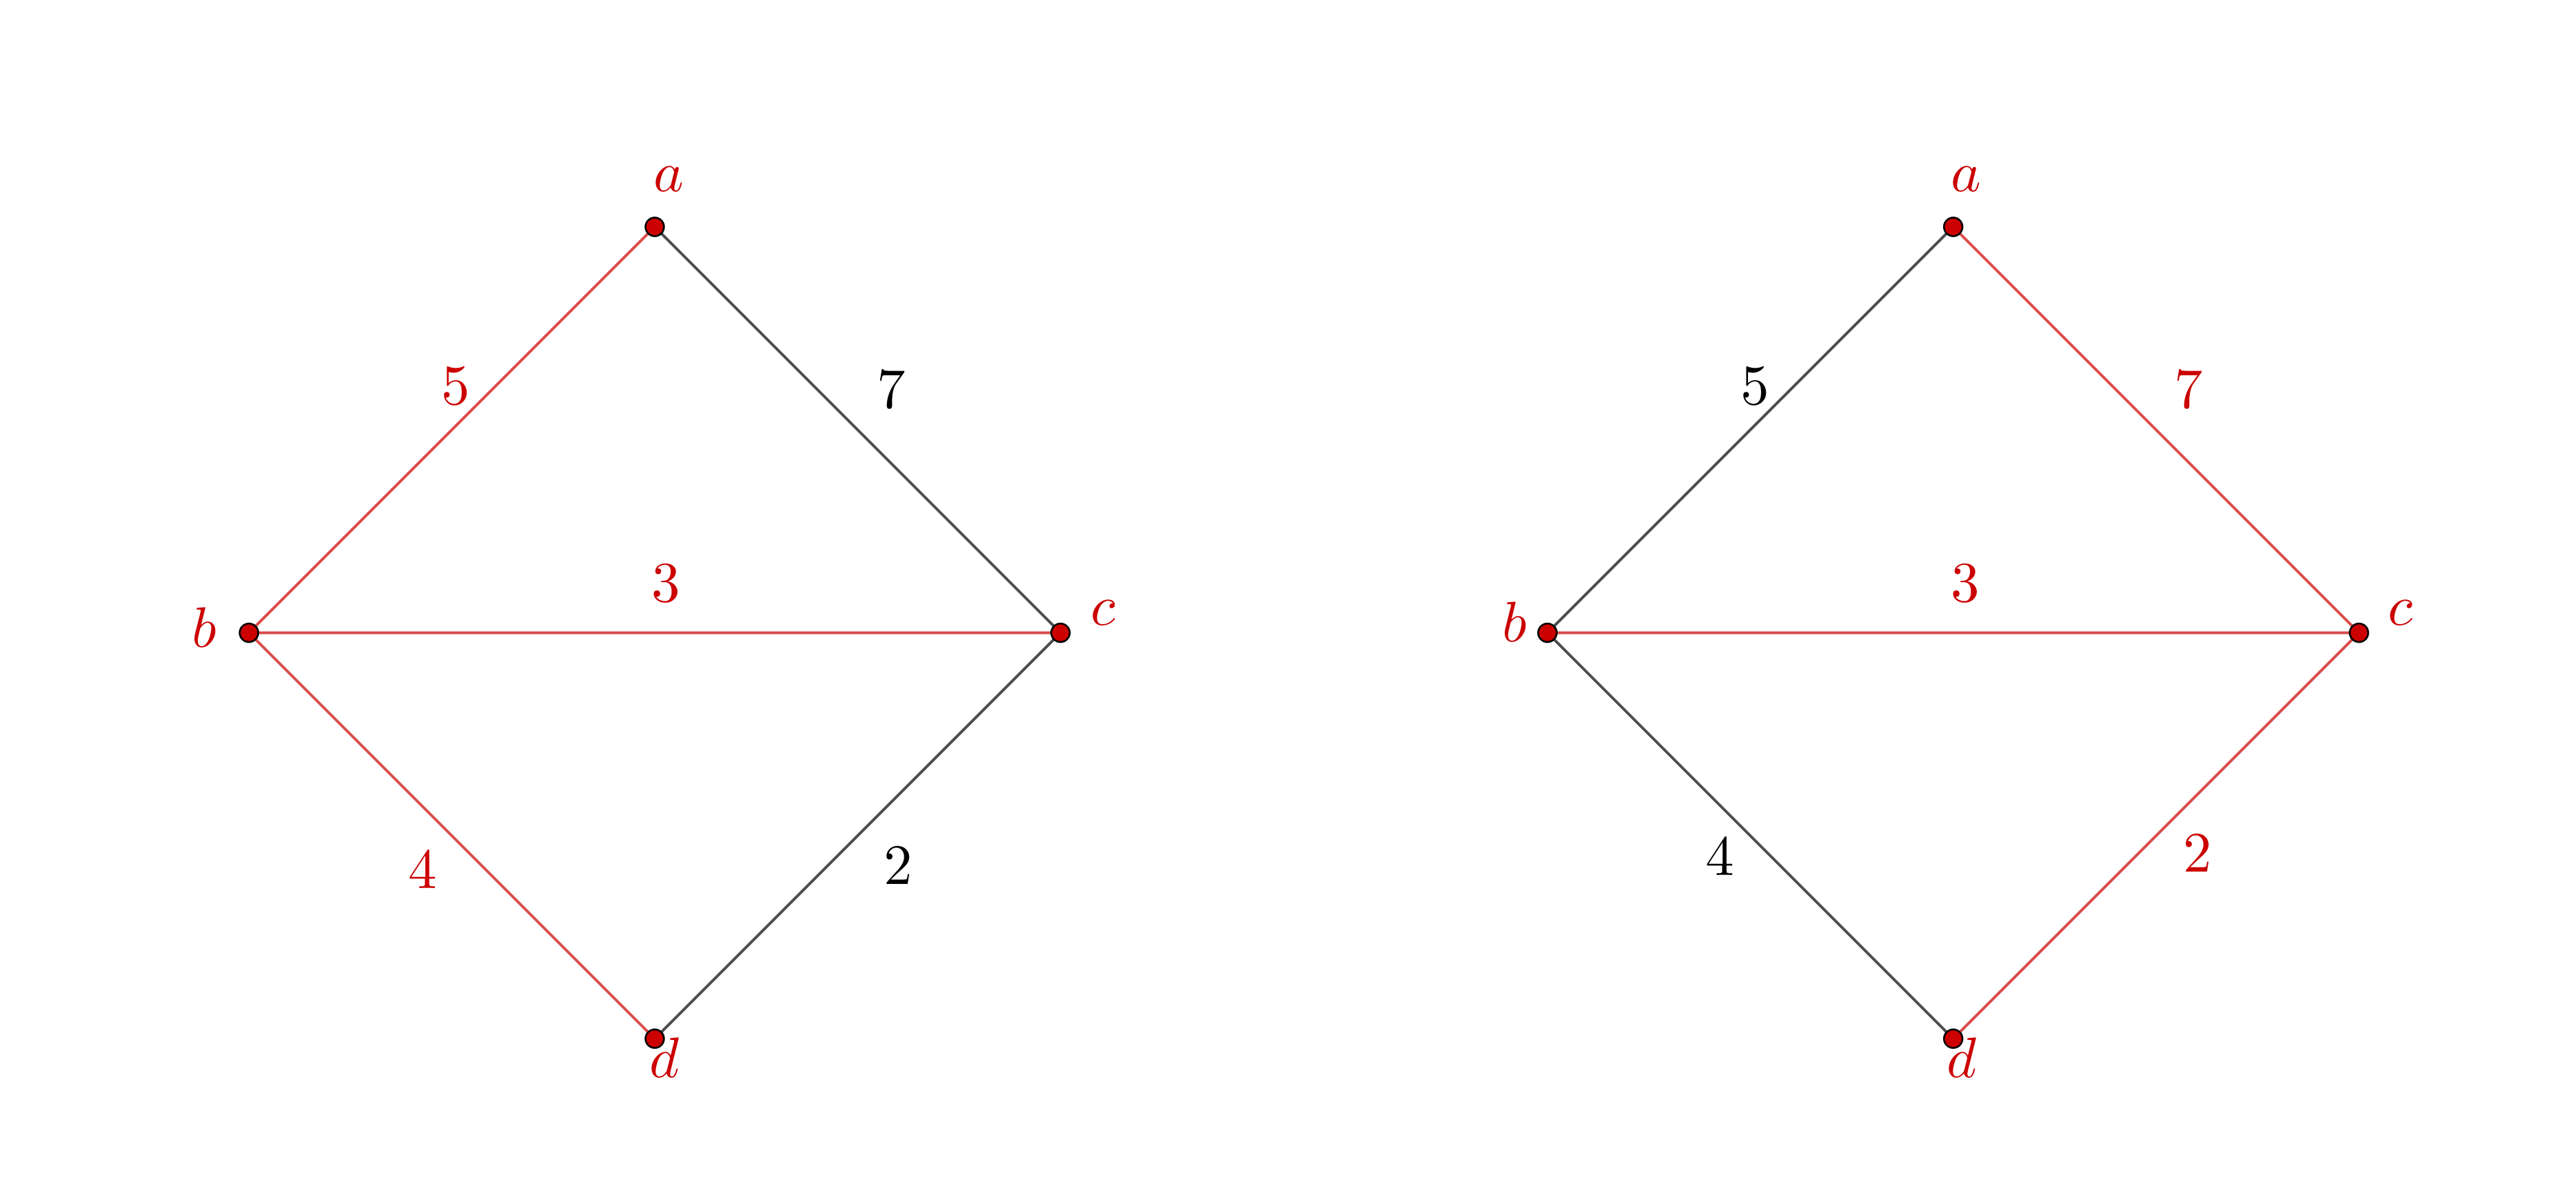
\includegraphics{graphics/L6_prim_kruskal_dijkstra/Ex_3_project.png}
       \caption{Counterexample for Exercise 3.}
    \label{ex_3}
\end{figure}
To see that this does not hold we can look at an example. Let $G=(V,E)$ be the graph for
$$V = \{a,b,c,d\}\quad\text{and}\quad E = \{ \{a,b\}, \{a,c\}, \{b,c\}, \{b,d\}, \{c,d\} \}.$$ 
We can choose spanning trees $T_1 = (V, E_1)$ and $T_2 = (V, E_2)$ with $E_1 = \{ \{a,c\}, \{b,c\}, \{c,d\} \}$ and $E_2=\{a,b\}, \{b,c\}, \{b,d\} \}$ (see Figure \ref{ex_3}). If we assign weights as shown in the figure we obtain a weight of 12 for both $T_1$ and $T_2$. Hence the statement is not true.



\section*{Exercise 4}
\emph{One way to find a path between two vertices is to first find a minimum spanning tree for the graph and then find the unique path between them in this tree. Will this always be the shortest path between them? If not, will there always be some pair of vertices such that this is the shortest path between them?}
\vspace{0.4cm}

The path in the tree between two vertices is not necessarily the shortest path between two vertices in the graph. To see that we can observe the same graph as in exercise 3. The minimum spanning tree is the tree $T = (V,E)$ for $V = \{a,b,c,d\}$ and $E = \{\{a,b\}, \{b,d\}, \{d,c\}\}$. The shortest path from $b$ to $c$ is simply the edge $\{b,c\}$ with weight 3, but the path in $T$ is the path $b,d,c$ that has weight 6.

Luckily, there will always be a pair of vertices such that the path in the tree is the shortest path between them. To see that we can take an edge $e \in E$ such that $w(e)$ is minimal among all edges. Choose this edge to be the first edge for creating an MST using Kruskal's algorithm. Thereby the edge $e$ must be included in a minimal spanning tree. By choosing the two vertices incident to the edge $e$ we obtain a pair of vertices for that the unique path in the tree is actually the shortest path.

\section*{Exercise 5}
\emph{Are any of the things we did in this lecture useful for computing the diameter of a graph? Think about how one might do it, and what runtimes your suggested algorithms will have.}
\vspace{0.4cm}

For any vertex $v$ of the graph $G$ we can use Dijkstra's algorithm to find the vertex with the largest distance to $v$ in $G$ by simply letting the algorithm visit all vertices and comparing the distances. We as such let $l(v) = max_{v' \in G} d(v, v')$. We note that for the runtime of computing $l(v)$ we apply Dijkstra’s algorithm and then find the largest value which takes $|E|$ steps. We therefore get for computing $l(v)$ the runtime $\mathcal{O}(|E| + |V|\log(|V|) + |E|) = \mathcal{O}(|E| + |V|\log(|V|))$. We can then apply this method to all vertices and find the largest distance between the vertices in the graph by taking $max_{v \in G} l(v)$, giving us the diameter of the graph. This method applies $l(v)$ $|E|$ times while comparing the values in $|E|$ steps. We therefore get a runtime of $\mathcal{O}(|E|(|E| + |V|\log(|V|)) + |E|) = \mathcal{O}(|E|^2 + |E||V|\log(|V|))$.


\end{document}
